%-------------------------------------------------------------------------------------------
	\section{Generic OS design for Heighway dragon}
%-------------------------------------------------------------------------------------------



We propose a generic design of deterministic oritatami system that allows us to fold an arbitrary finite portion of the Heighway dragon. 
%The design concept has been already explained in the introduction. 
The folded dragon is actually slanted as illustrated in Fig.~\ref{fig:heighway6_oritatami}, which is more natural than the conventional (upright) one to be folded over the triangular grid. 
%Let $P[j_1 .. j_2]$ be the target portion and $n = \min\{m \mid j_2 < 2^m\}$. 
Independently of which portion to be folded, the design sets both delay and arity to 3 and employs 567 bead types and a fixed rule set $\mathcal{H}$ (some of the bead types could be saved but not easily due to the NP-hardness of saving \cite{HanKim2017}). 
It also challenges to make the resulting OS cyclic. 
Otherwise one could simply design left and right-turn modules and concatenate their copies according to the (non-periodic) sequence $P$. 
Such a ``hardcoding'' however goes against the spirit of algorithmic self-assembly, and an OS that folds into the infinite Heighway dragon, if any, could not take this approach in order to be describable by a finite mean. 

%Any finite portion of the Heighway dragon is expected to be foldable by \textit{hard-coding} if an arbitrary number of bead types is available and the shape can be scaled-up (though, if rescaling is not allowed, it is NP-hard to decide if for a given finite shape, there exists an oritatami system that folds into the shape \cite{PatitzRogers2017}). 
%The proposed design cannot take this approach because the number of bead types available is fixed. 
%An oritatami system $\Xi = (\mathcal{H}, \alpha, \delta, \sigma, w)$ that the design provides is periodic in the sense that its transcript is a periodic sequence. 
%If this system is for the $n$-th repetition of the Heighway dragon, then the length of its period is $|w|/2^{n-1}$. 
%One period corresponds to a successive two pairs of a red line segment and the following green L-shaped block. 

One period folds into successive two line segments of the dragon. 
Why does the design distinguish them? 
The answer lies in that the dragon is slanted. 
The slanted dragon involves two types of left turn as well as two types of right turn: acute and obtuse. 
%Capability of one turning module to make all of the four possible turns would halve the period. 
%Such a turning module, however, would have to take quite a number of conformations; recall that what the module has to turn is not a straw but a thick wire through which the current count $i$ propagates. 
Capability of one turning module to make all of the four possible turns would halve the period but require quite a number of conformations. 
Recall that what the module has to turn is not a straw but a thick wire through which the count $i$ propagates. 
Such a module is too advanced for the current oritatami technology.  
Our approach makes it enough for a turning module to handle just two tasks: turning acutely and turning obtusely. 
%Observe that after (slanted) vertical segments, the left turn is obtuse while the right turn is acute, whereas after horizontal ones, the left turn is acute while the right turn is obtuse. 
Observe that after (slanted) vertical segments, the dragon turns left obtusely and right acutely, whereas after horizontal ones, it turns left acutely and right obtusely. 
Moreover, vertical and horizontal segments alternate on the dragon. 
%Hence, we can attach a proper interpreter \textit{a priori} to each DFAO module to convert its output L/R into a signal A(cute)/O(btuse). 
Thus, each segment can be equipped with a proper interpreter \textit{a priori} of the direction L/R into a signal A(cute)/O(btuse) using two types of interpreters: the vertical one interprets L as O and R as A, while the horizontal one does conversely. 

\begin{figure}[tb]
\centering
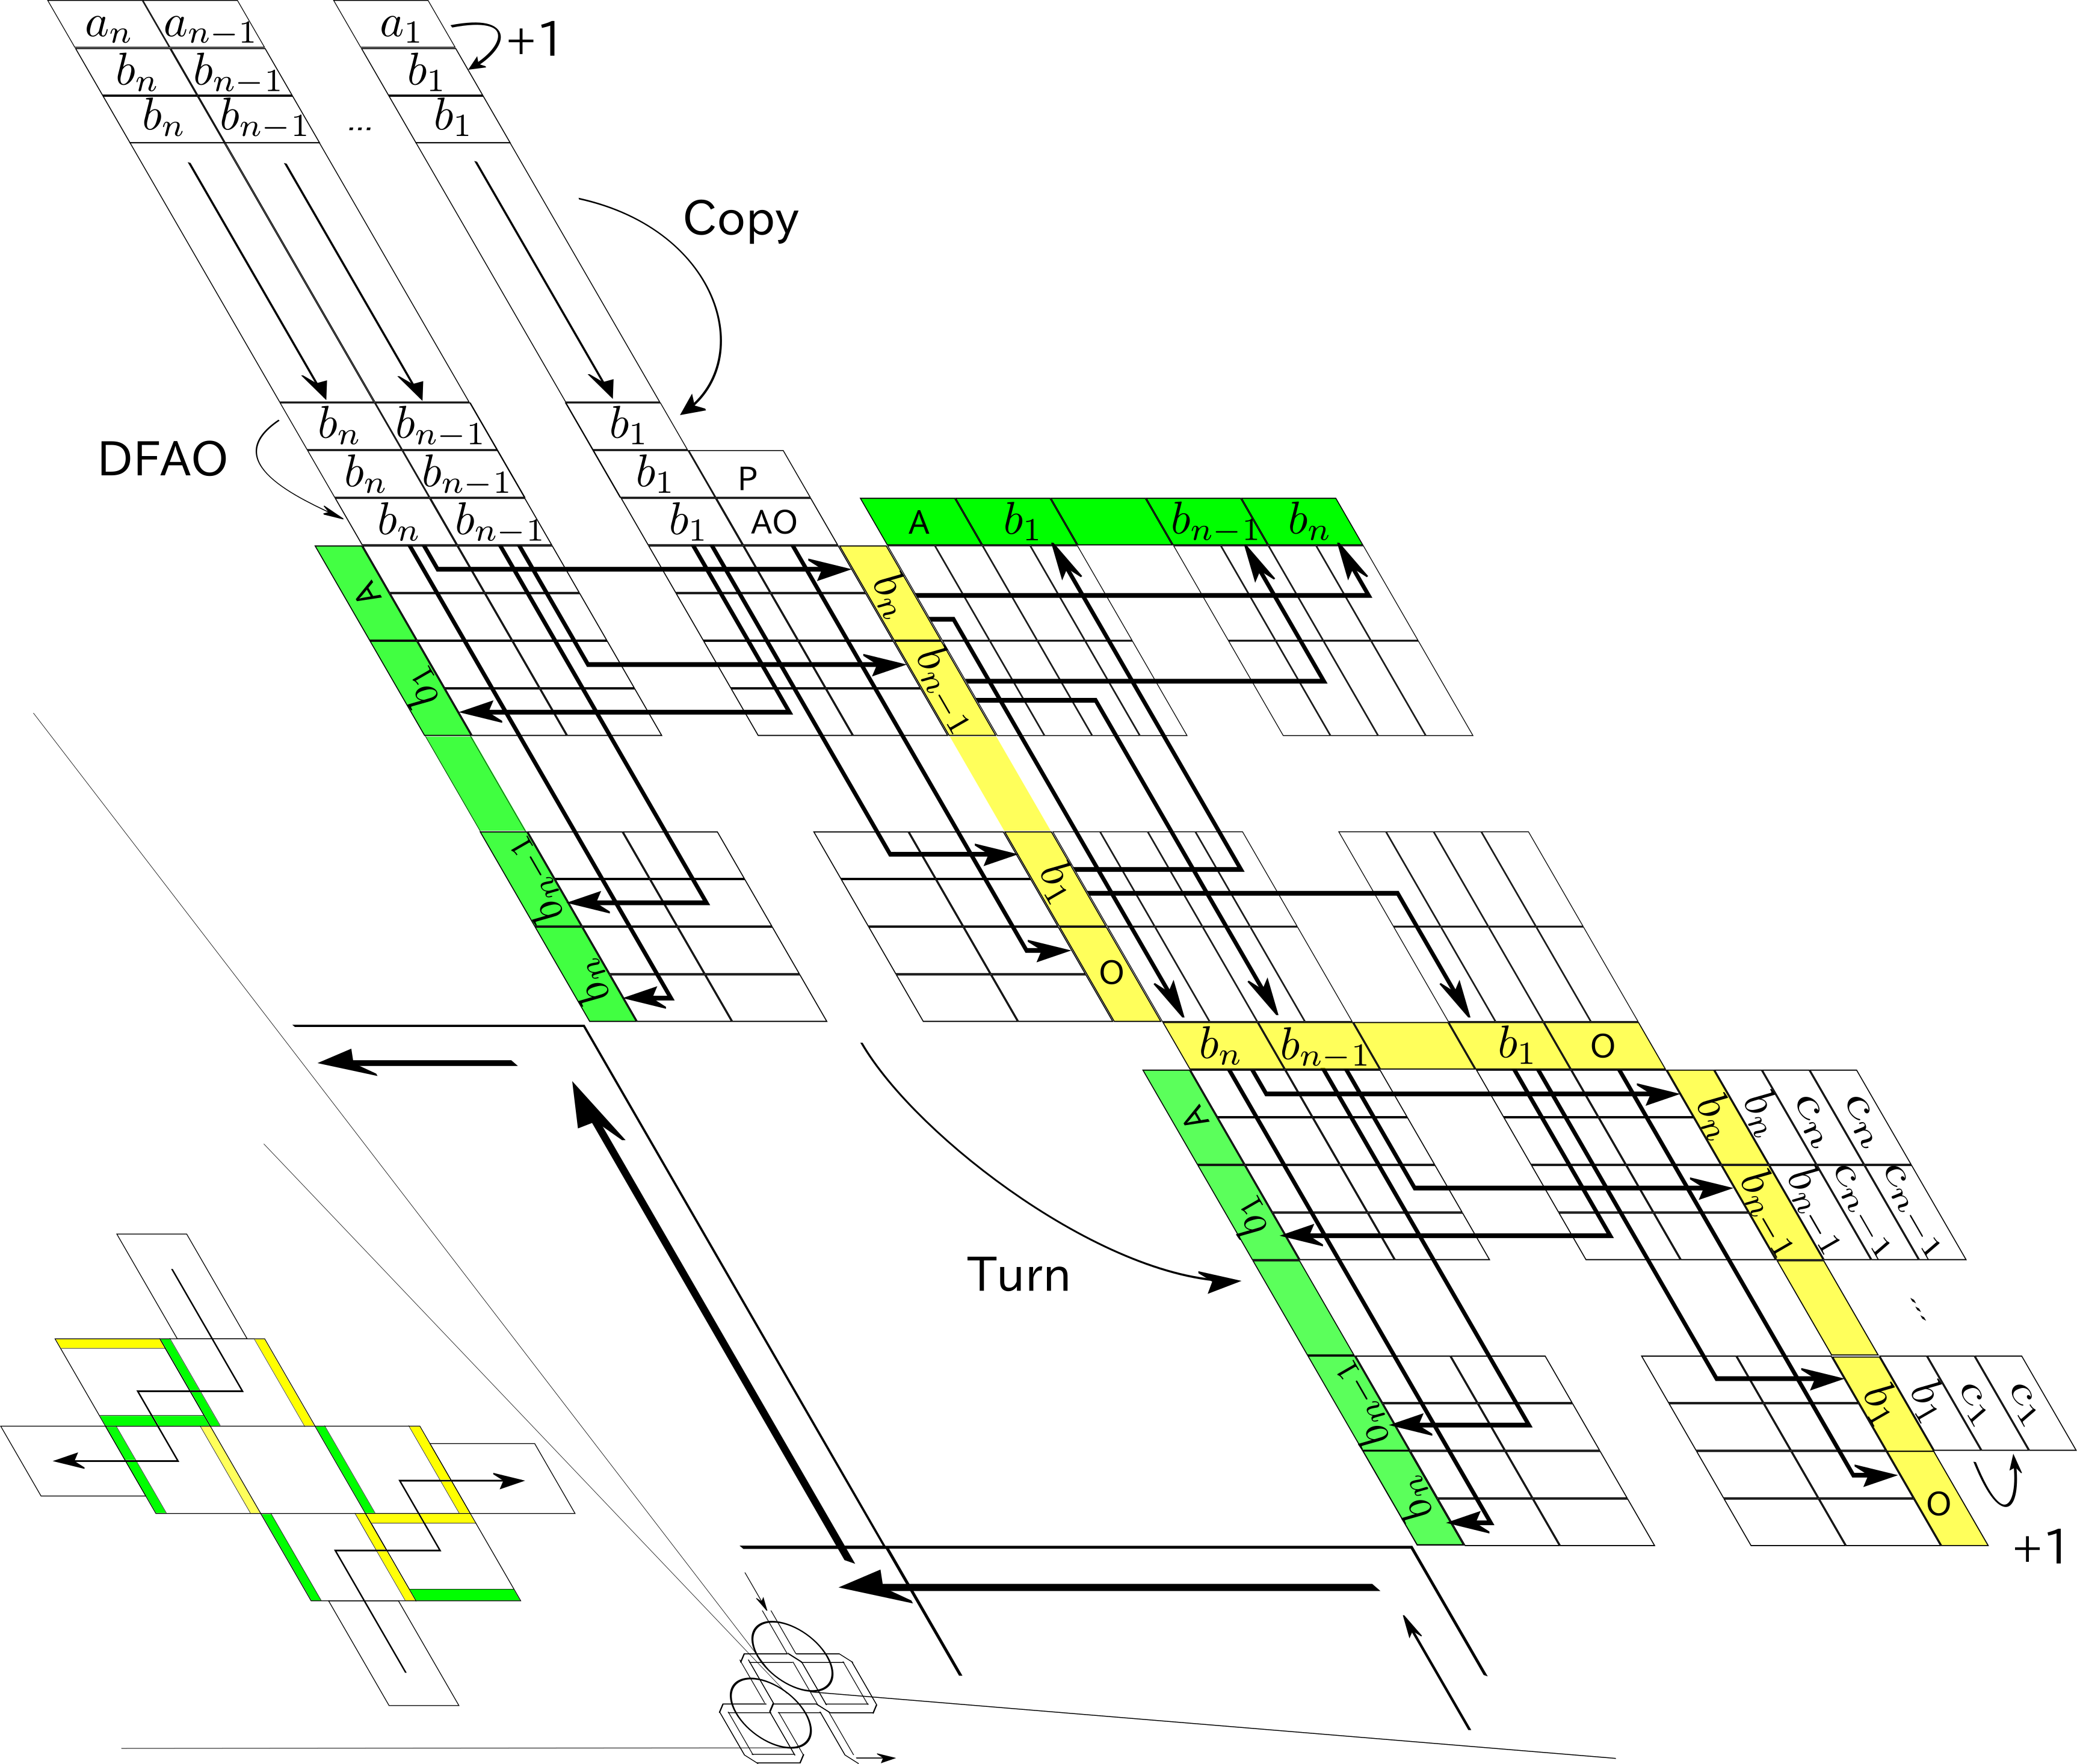
\includegraphics[width=0.8\linewidth]{pic/dragon_vol5.png}
\caption{
Folding of one segment plus turn of the Heighway dragon, flow of information through it, and the two ways of collision avoidance between two turns.
}
\label{fig:abst_dragon}
\end{figure}

The first and second halves of a period differ only in the type of interpreter (AO or $\overline{\rm AO}$) so that we just explain the first. 
%Its transcript consists of three subsequences respectively for the counters, DFAO, and turning modules. 
%It folds as abstracted in Fig.~\ref{fig:abst_dragon} into one line segment plus one turn of the dragon and has its three subsequences accomplish the following tasks, respectively: 
Its transcript folds as abstracted in Fig.~\ref{fig:abst_dragon} into one line segment plus one turn of the dragon. 
The transcript consists of three subsequences (modules) responsible for the following tasks, respectively:  
\begin{enumerate}[itemsep=0pt]
\item (Counter module) $i \gets i + 1$ and propagate $i$, drawing a line segment;
\item (DFAO module) Compute $P[i]$ and interpret it properly as A or O;
\item (Turning module) Make a turn accordingly.
\end{enumerate}
%The length of the half is proportional to $n^2$ and hence so is that of a period. 
%The seed of the system replaces the first counter module of the first period and encodes the initial count $j_1$ as a sequence of bead types in a format that the following counters can ``read.'' 
%We shall explain how something is read later. 
Before explaining them, one issue intrinsic to the folding by oritatami systems should be pointed. 
It rises when the dragon makes a turn where it has already turned before. % that is, when two turns share a point. 
By definition, OSs cannot put a bead anywhere occupied by another bead. 
Being scaled sufficiently large, a rhombus corresponding to a point affords two turning modules, which otherwise collide, as long as they fold into an L-shape (Figs.~\ref{fig:heighway6_oritatami} and \ref{fig:abst_dragon}). 
A turning module has its three bifurcator submodules direct further folding obtusely one after another guided by the signal O from the previous DFAO module, as colored in yellow in Figs.~\ref{fig:abst_dragon}, \ref{fig:PFS}, \ref{fig:change_route}, or acutely one after another by A, as colored in green, and folds into two L-shape conformations. 
Note that two turns which share a point are both acute or both obtuse. 

%-------------------------------------------------------------------------------------------
		\subsubsection{Modules}
%-------------------------------------------------------------------------------------------

Having outlined the generic design, now we explain how the design implements an OS for a specific target portion $P[j_1 .. j_2]$, or more precisely, how the three modules of the OS and their components are implemented, interlocked with each other, and collaborate. 
%Now we explain how modules and their components have been implemented, interlocked with each other, and collaborate. 
Let $n = \min\{m \mid j_2 < 2^m\}$. 
The counter and turning modules, or more precisely, their transcripts, are of length $O(n^2)$ while the DFAO module is of length $O(n)$. 
Thus, the period of the OS is of length proportional to $n^2$. 
They consist of components of constant size. 
Using a simulator developed for \cite{HaKiOtSe2016}, we verified that all of the components fold correctly in all possible environments, which are abstracted in Figs.~\ref{fig:abst_dragon}, \ref{fig:abst_dfao}, and \ref{fig:overall_turning}. 

%-------------------------------------------------------------------------------------------
			\paragraph{Counter module}
%-------------------------------------------------------------------------------------------
%
We have modified the existing binary counter \cite{GeMeScSe2016} so as to operate in the dynamics \eqref{eq:cotranscriptional_folding}, which is more prevailing \cite{HanKim2017,HaKiOtSe2016,OtaSeki2017} though less tractable. 

%%%%%%%%%%%%%%%%%%%%%%%%%%%%%%%%%%%%%%%%%%%%
%\begin{figure}[h]
\begin{wrapfigure}{r}{0.6\linewidth}
\vspace*{-5mm}
\centering
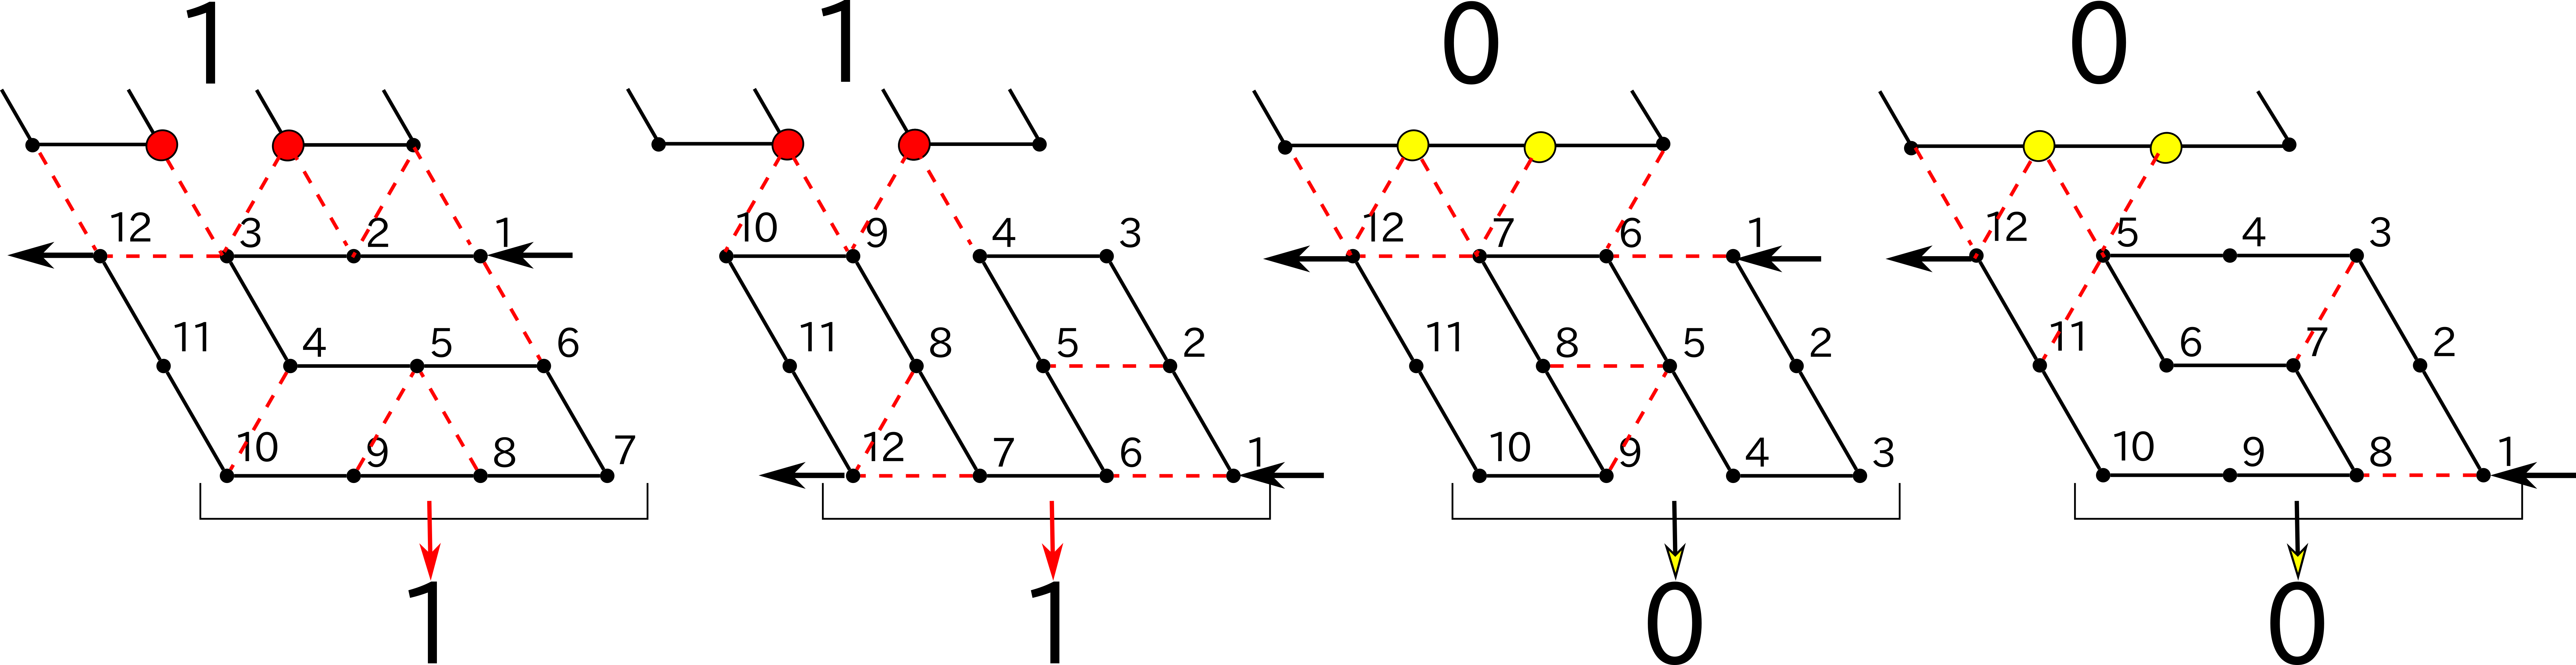
\includegraphics[width=\linewidth]{pic/counter_zig.png}
\caption{All conformations of the half-adder.
The first and third are diverted to implement the body-lpx2 component of the turning module. 
}
\label{fig:half-adder}
\vspace*{-5mm}
\end{wrapfigure}
%\end{figure}
%%%%%%%%%%%%%%%%%%%%%%%%%%%%%%%%%%%%%%%%%%%%

A counter module for $n$-bit sequences is a catenation of the following components in the order: right-turner, $n$ half-adders, left-turner, and $n$ formatters. 
It folds into one zigzag (throughout the paper, zig means going leftward and zag means rightward). 
Suppose each bit of an $n$-bit input $a_n a_{n-1} \cdots a_1$ is encoded as a specific sequence of 4-bead types ({\tt HA-1} for 1 and {\tt HA-0} for 0) as suggested in Fig.~\ref{fig:half-adder} and the input is provided as the catenation of such bit sequences for $a_n, a_{n-1}, \ldots, a_1$. 
The right-turner folds so as for the first bead of the first half-adder to come at a distance of either 1 or 3 southeastward from the rightmost bead of the LSB $a_1$. 
Thus, the first half-adder encounters only the four surrounding environments (contexts) shown in Fig.~\ref{fig:half-adder}, in which the transcript {\tt 1}-{\tt 2}-\dots-{\tt 12} of half-adder folds deterministically as illustrated, or more precisely, the generic rule set $\mathcal{H}$ is designed so as for the transcript to favor the illustrated conformation the most in each context. 
Interpreting the first bead {\tt 1} (resp.~last bead {\tt 12}) being far from the input as carry-in (resp.~carry-out) and close as no carry-in (resp.~no carry-out), we can see carry be out only when $a_1$ is 1 and carried in (the second context in Fig.~\ref{fig:half-adder}). 
Being concatenated, half-adders ripple carry from one to the other. 
The half-adder can expose four sequences below: {\tt HA-1a}, {\tt -0a}, {\tt -0b}, and {\tt -1b} as output. 
They are pairwise distinct enough for a formatter, which is supposed to come below in the next zag, guided by the left-turner, to favor one conformation below {\tt HA-1a}/{\tt 1b} or the other  below {\tt HA-0a}/{\tt 0b}, which expose {\tt HA-1} and {\tt HA-0} downward, respectively. 
%They are pairwise distinct enough for another component to ``read'' the output. 
%After the left-turner guides the counter module from its zig to zag, $n$ formatters format each bit as {\tt HA-1a/1b} $\to$ {\tt HA-1} and {\tt HA-0a/0b} $\to$ {\tt HA-0} using its two conformations. 
Thus, a counter module increments an input by 1 if its first half-adder is fed with carry (i.e., the right-turner locates its {\tt 1} away from $a_1$), or just propagates it otherwise. 
The output and input are in the same format (1 as {\tt HA-1} and 0 as {\tt HA-0}) so that counter modules can be interlocked. 
Concatenating counter modules and feeding carry-in only to the first one yields a line segment through which the current count $i$ is incremented by 1 and propagated. 
The first counter module of the first period is replaced by the seed of the OS, which encodes the initial count $j_1$. 

\begin{comment}
A counter module folds into one zigzag. 
Its essential component is the half-adder. 
The first half of its transcript is a catenation of $n$ half-adders. 
In Fig.~\ref{fig:abst_dragon}, half-adders are abstracted as small parallelograms at the top labeled with $a_n$, $a_{n-1}$, $\ldots$, $a_1$, where the one with $a_j$ is for the $j$-th bit of the current count $i$. 
%Though not described, two horizontally adjacent half-adders sandwitch a glider of even length as a space to keep them away from each other sufficiently to prevent any undesirable interference. 
As illustrated in Fig.~\ref{fig:half-adder}, the whole system is designed in such a manner that a half-adder starts folding at one of two positions (top/bottom) relative to the 1-bit input (0/1) that is encoded as a sequence of bead types colored in red or yellow and it folds into one of the four possible conformations. 
Starting at the bottom should be interpreted as carry-in while at the top as no carry-in, and the position of ending should be interpreted analogously for carry-out. 
%The whole system is designed in such a manner that a 1-bit input (1 or 0) is exposed to the specific position (colored red or yellow in Fig.~\ref{fig:half-adder}) as a pair of bead types by the previous turning module. 
%The system is also designed in such a manner that a half-adder starts folding either at the top, as in the first and third conformations, or at the bottom as in the other two. 
%The half-adder considers starting at the top as non-carry and at the bottom as carry. 
%Thus, only when a half-adder takes 1 and carry, it ends at the bottom (second conformation in Figure~\ref{fig:half-adder}), which is propagated to the next half-adder as it is via the spacer between them. 
These four conformations expose sequences of four bead types below that are distinct enough to convey the intended 1-bit output to another computing component, or in other words, we can design a component that can ``read'' the output. 
From this point forward, conformations for other components will be illustrated; their input and output will be labeled by their meaning mutually understood by the components that exchange them. 
Observe that a half-adder can output 1 in two different formats {\tt HA-1a} and {\tt HA-1b} and also 0 as {\tt HA-0a} and {\tt HA-0b}. 
The role of the zag is to reformat them into {\tt HA-1} and {\tt HA-0} so that other components can read them easily. 
A counter module either increments an input by 1 if being fed with carry, or propagates the input otherwise. 
%Being fed with non-carry, the counter module serves as the copier module. 
\end{comment}

%-------------------------------------------------------------------------------------------
			\paragraph{DFAO module}
%-------------------------------------------------------------------------------------------
%
As abstracted in Fig.~\ref{fig:abst_dfao}, a DFAO module receives the current count $i$ from the previous counter module, computes $P[i]$, interprets it properly either A or O, and outputs it together with the count $i$. 

\begin{figure}[tp]
\centering
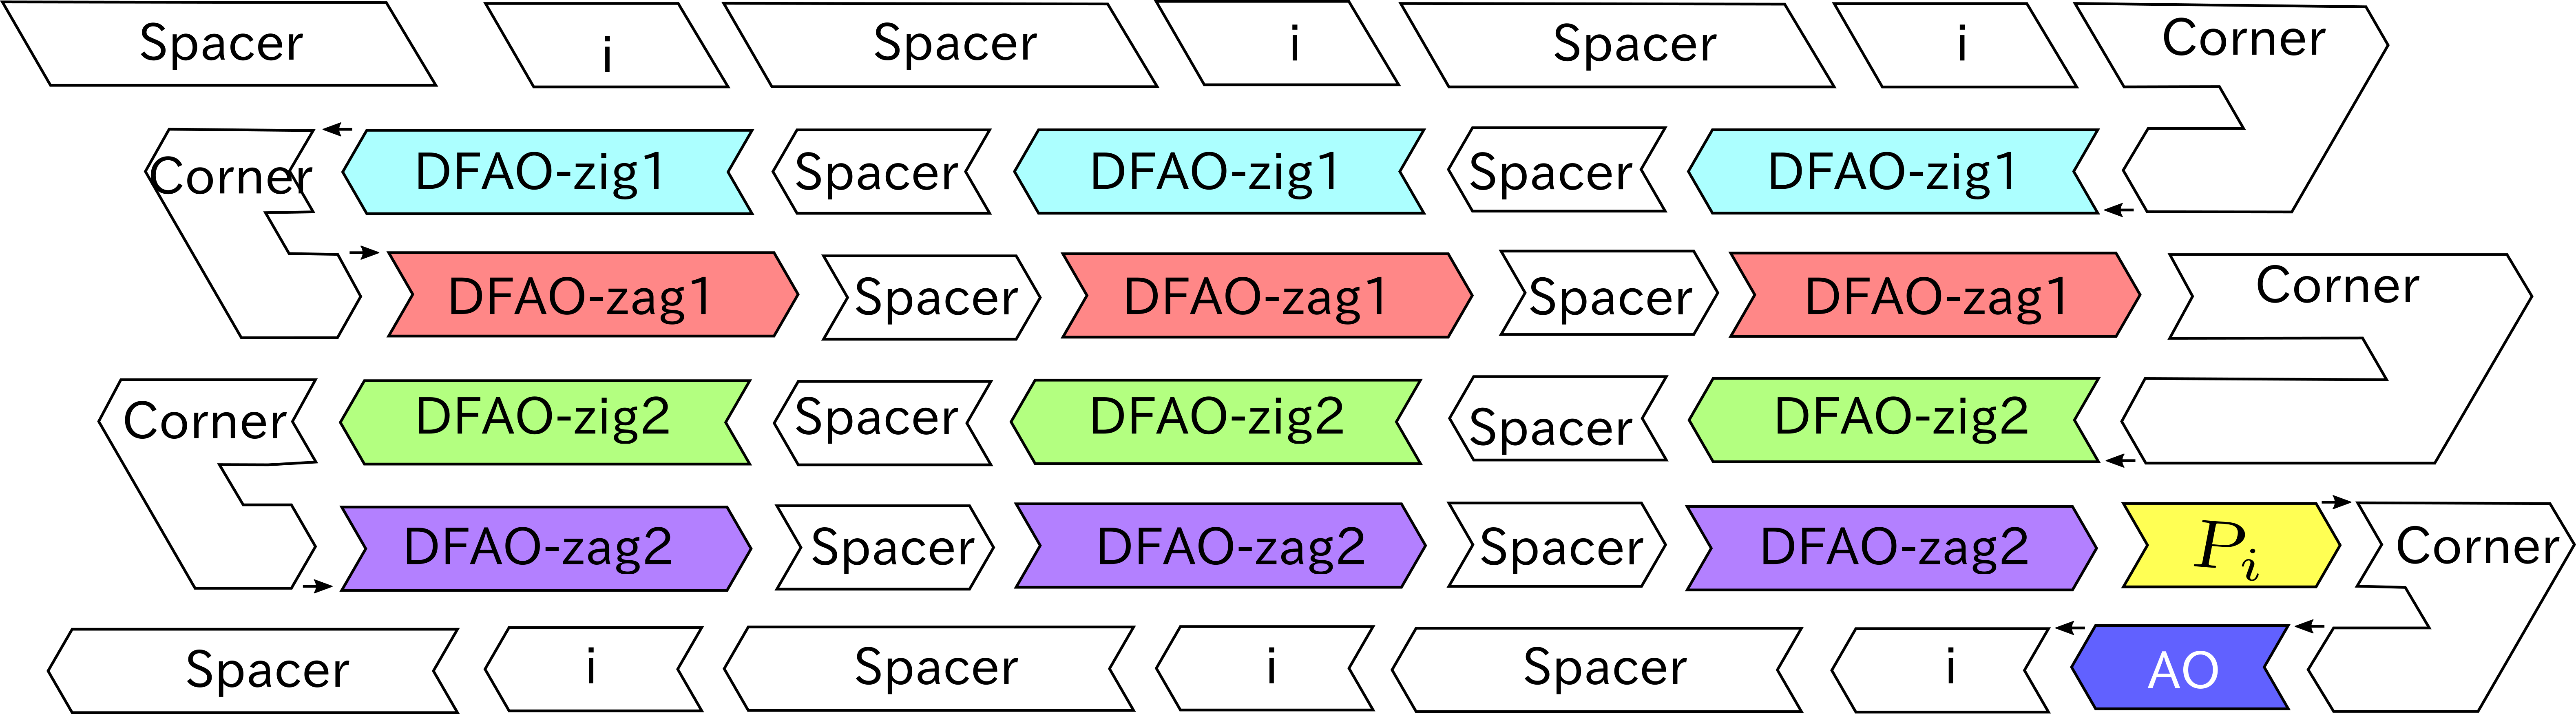
\includegraphics[width=0.8\linewidth]{pic/abst_DFAO.png}
\caption{Component-level abstraction of the folding of DFAO module.}
\label{fig:abst_dfao}
\end{figure}

%%%%%%%%%%%%%%%%%%%%%%%%%%%%%%%%%%%%%%%%%%%%

\begin{figure}[h]
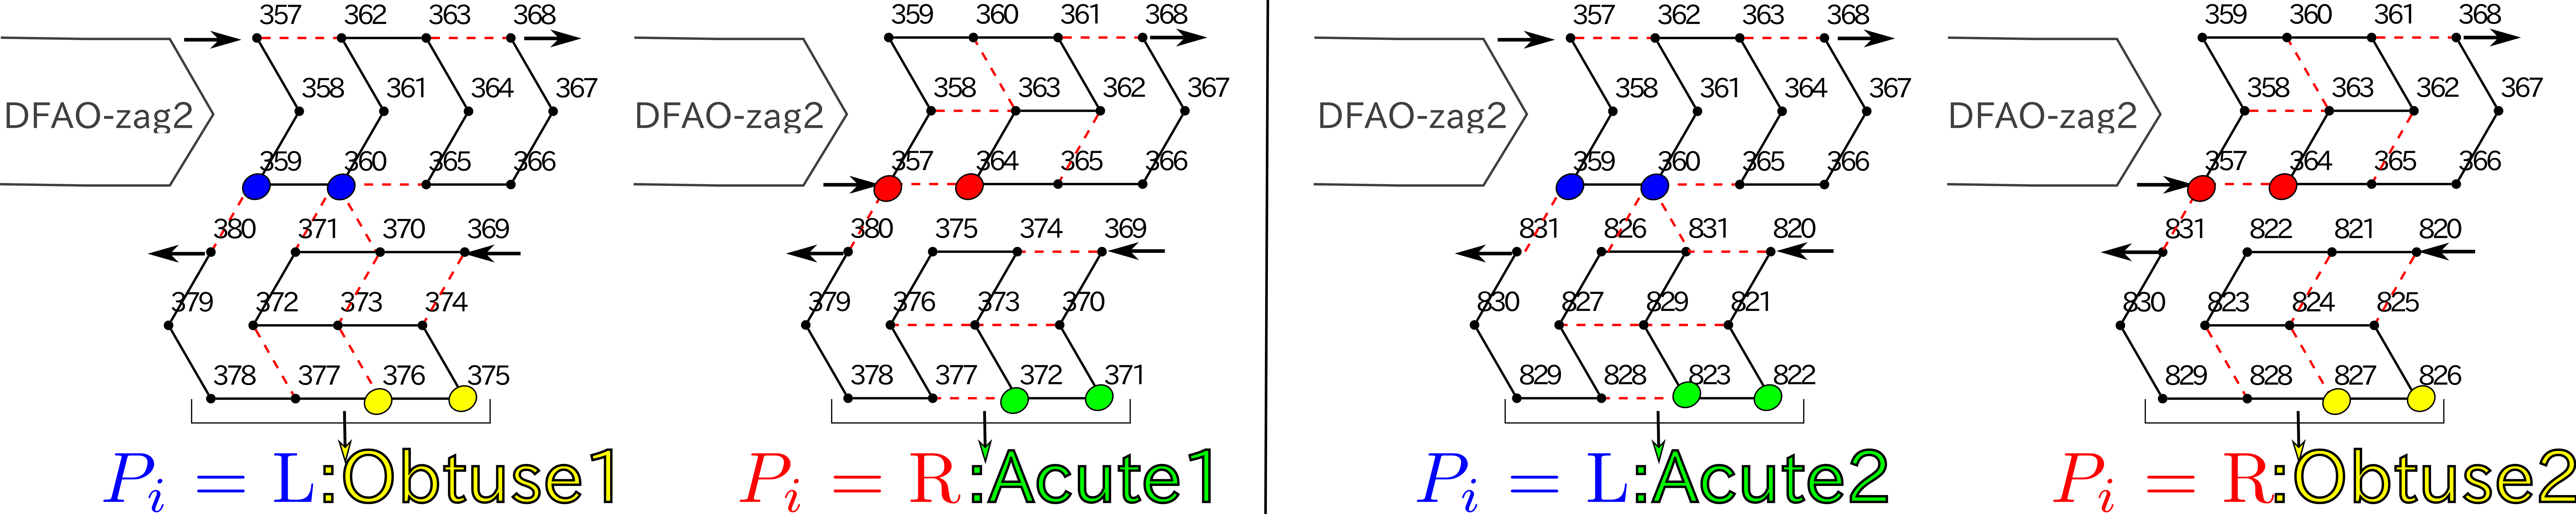
\includegraphics[width=\linewidth]{pic/PFS.png}
\caption{The two conformations of PFS above and the corresponding two conformations of (left) AO and (right) of $\overline{\rm AO}$.}
\label{fig:PFS}
\end{figure}
%%%%%%%%%%%%%%%%%%%%%%%%%%%%%%%%%%%%%%%%%%%%

Observe in Fig.~\ref{fig:heighway_dragon} that what the DFAO does exactly in order to compute $P[i]$ is to search for the first 0 read from the LSB and check whether it is followed by 0 ($P[i] = {\rm R}$) or by 1 ($P[i] = {\rm L}$). 
%While folding into zigzag twice and one more zig (see Fig.~\ref{fig:abst_dfao}), the DFAO module does the search and check in the first and second zigzags, respectively.
See Fig.~\ref{fig:abst_dfao}. 
The DFAO module employs the following six components: DFAO-zig1, -zag1, -zig2, -zag2, PFS, and AO (or $\overline{\rm AO}$). 
It folds into one zigzag for the search and one more zigzag for the check. 
%The DFAO module is composed of the six components: DFAO-zig1, DFAO-zag1, DFAO-zig2, DFAO-zag2, PFS, and AO (or  ``$\overline{\rm AO}$").
%It folds into two zigzags and one more zig.
%In the first zigzag, DFAO-zig1s and -zag1s read $i$ from its LSB and ``mark" the first 0. 
%In the second zigzag, DFAO-zig2s and -zag2s check whether the marked 0 is followed by 0 ($P[i] = L$) or 1 ($P[i] = R$) and have PFS output $P[i]$ downward (see Fig.~\ref{fig:PFS} also for AO and $\overline{\rm AO}$). 
It folds into one more zig, in which, as shown in Fig.~\ref{fig:PFS}, AO interprets the output L of PFS as obtuse and R as acute if this module is for a vertical segment, or $\overline{\rm AO}$ interprets them the other way around otherwise. 
%The last zig is equipped with AO if this module is for a vertical segment or with $\overline{\rm AO}$ otherwise; as shown in Fig.~\ref{fig:PFS}, AO interprets the output L of PFS as obtuse and R as acute, while $\overline{\rm AO}$ interprets them the other way around. 

%%%%%%%%%%%%%%%%%%%%%%%%%%%%%%%%%%%%%%%%%%%%
%\begin{figure}[h]
\begin{wrapfigure}{r}{0.65\linewidth}
\vspace*{-5mm}
\centering
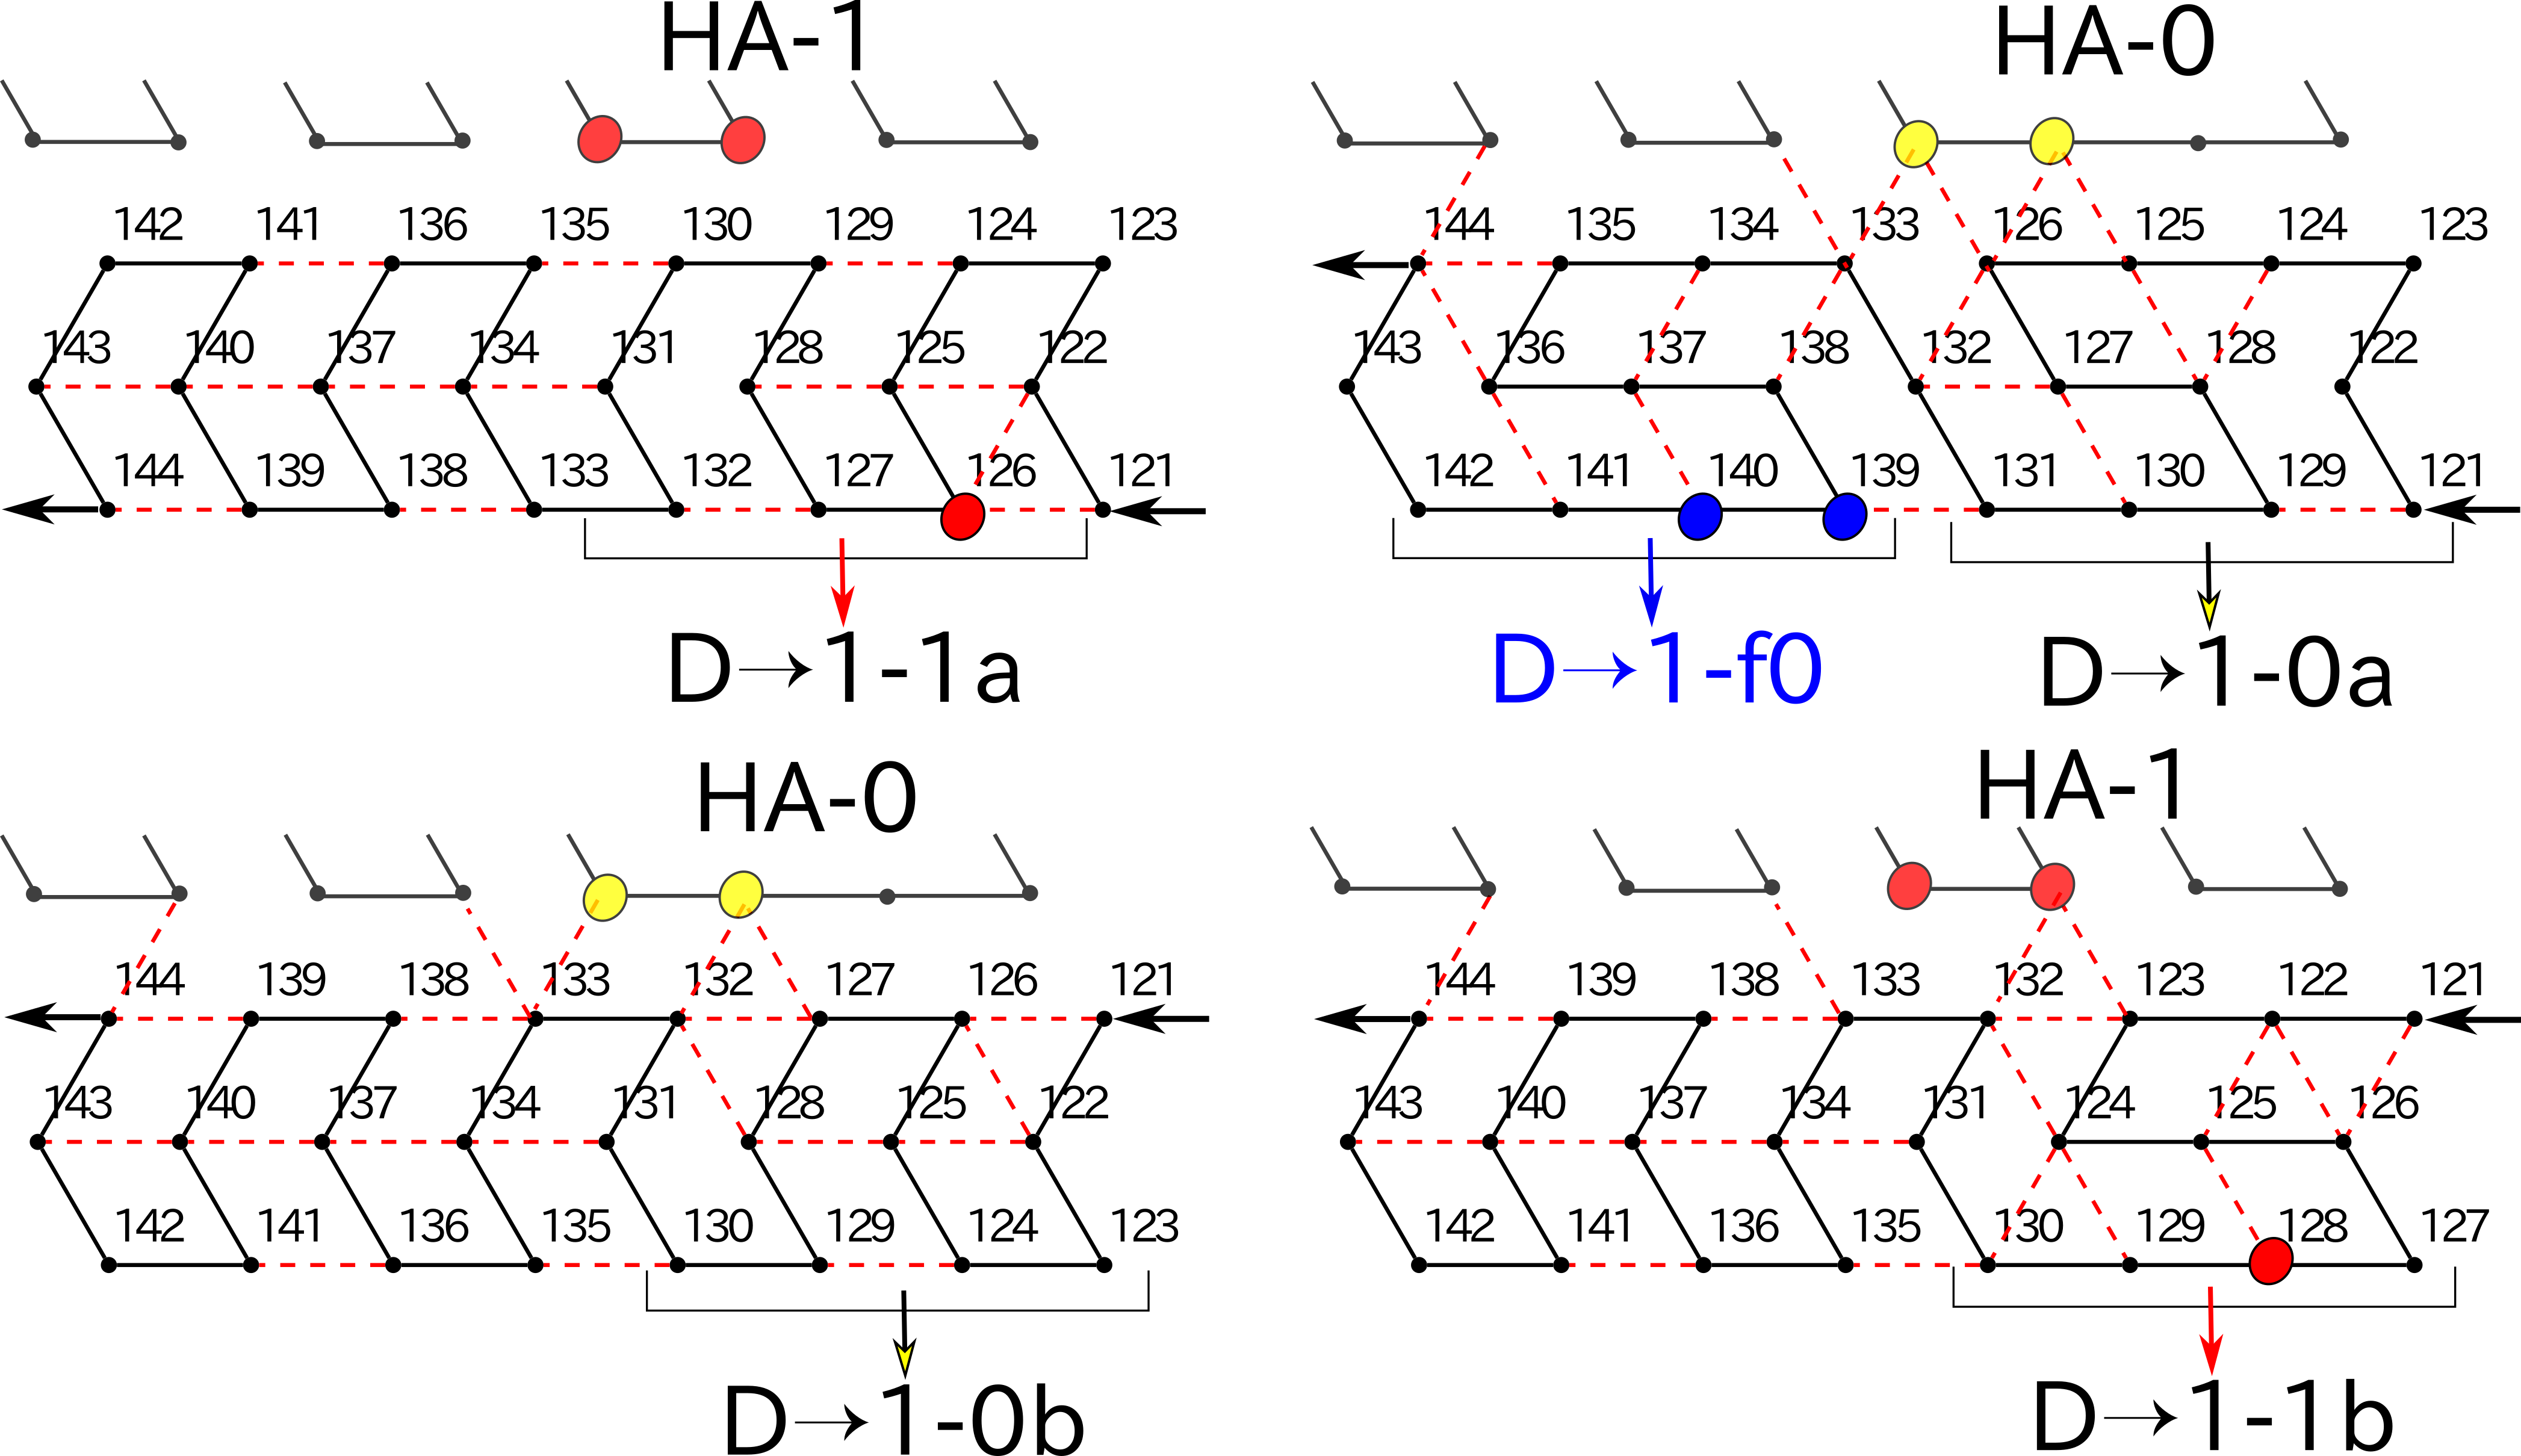
\includegraphics[width=\linewidth]{pic/DFAO-zig1.png}  
\caption{The four conformations of DFAO-zig1: (top) Dzig1-1 and Dzig1-f0; (bottom) Dzig1-20 and Dzig1-21.}
\label{fig:DFAO-zig1}
\vspace*{-3mm}
\end{wrapfigure}
%\end{figure} 

Since the count $i$ is $n$-bit, $n$ DFAO-zig1s are catenated and detect the first 0 collaboratively in two phases.
See Fig.~\ref{fig:DFAO-zig1} for its possible contexts and corresponding conformations. 
Phase1 is to copy all the 1's prior to the first 0 and Phase2 is to copy all the bits after the first 0.
These phases are distinguished by the relative position where a DFAO-zig1 starts folding to the input (far in Phase~1 while close in Phase~2).
In Phase1, DFAO-zig1s certainly take the conformation Dzig1-1 (the top left one in Fig.~\ref{fig:DFAO-zig1}).
At the first 0, a DFAO-zig1 folds into Dzig1-f0 instead, ending at the top in order to transition to Phase~2.
Each of the succeeding DFAO-zig1s takes Dzig1-20 or -21 to copy all the remaining bits. 
Note that there is a cushion between two DFAO-zig1s called \textit{spacer}.
Spacers are used to prevent undesirable interference among components.
They are implemented as a glider (see Sect.~\ref{sect:preliminaries}), hence capable of propagating 1bit on which phase the system is in.
In the first zag, $n$ DFAO-zag1s reformat and propagate 0's, 1's, and the first 0 using conformations in Fig.~\ref{fig:DFAO-zag1}.




%%%%%%%%%%%%%%%%%%%%%%%%%%%%%%%%%%%%%%%%%%%%%%%%
\begin{figure}[h]
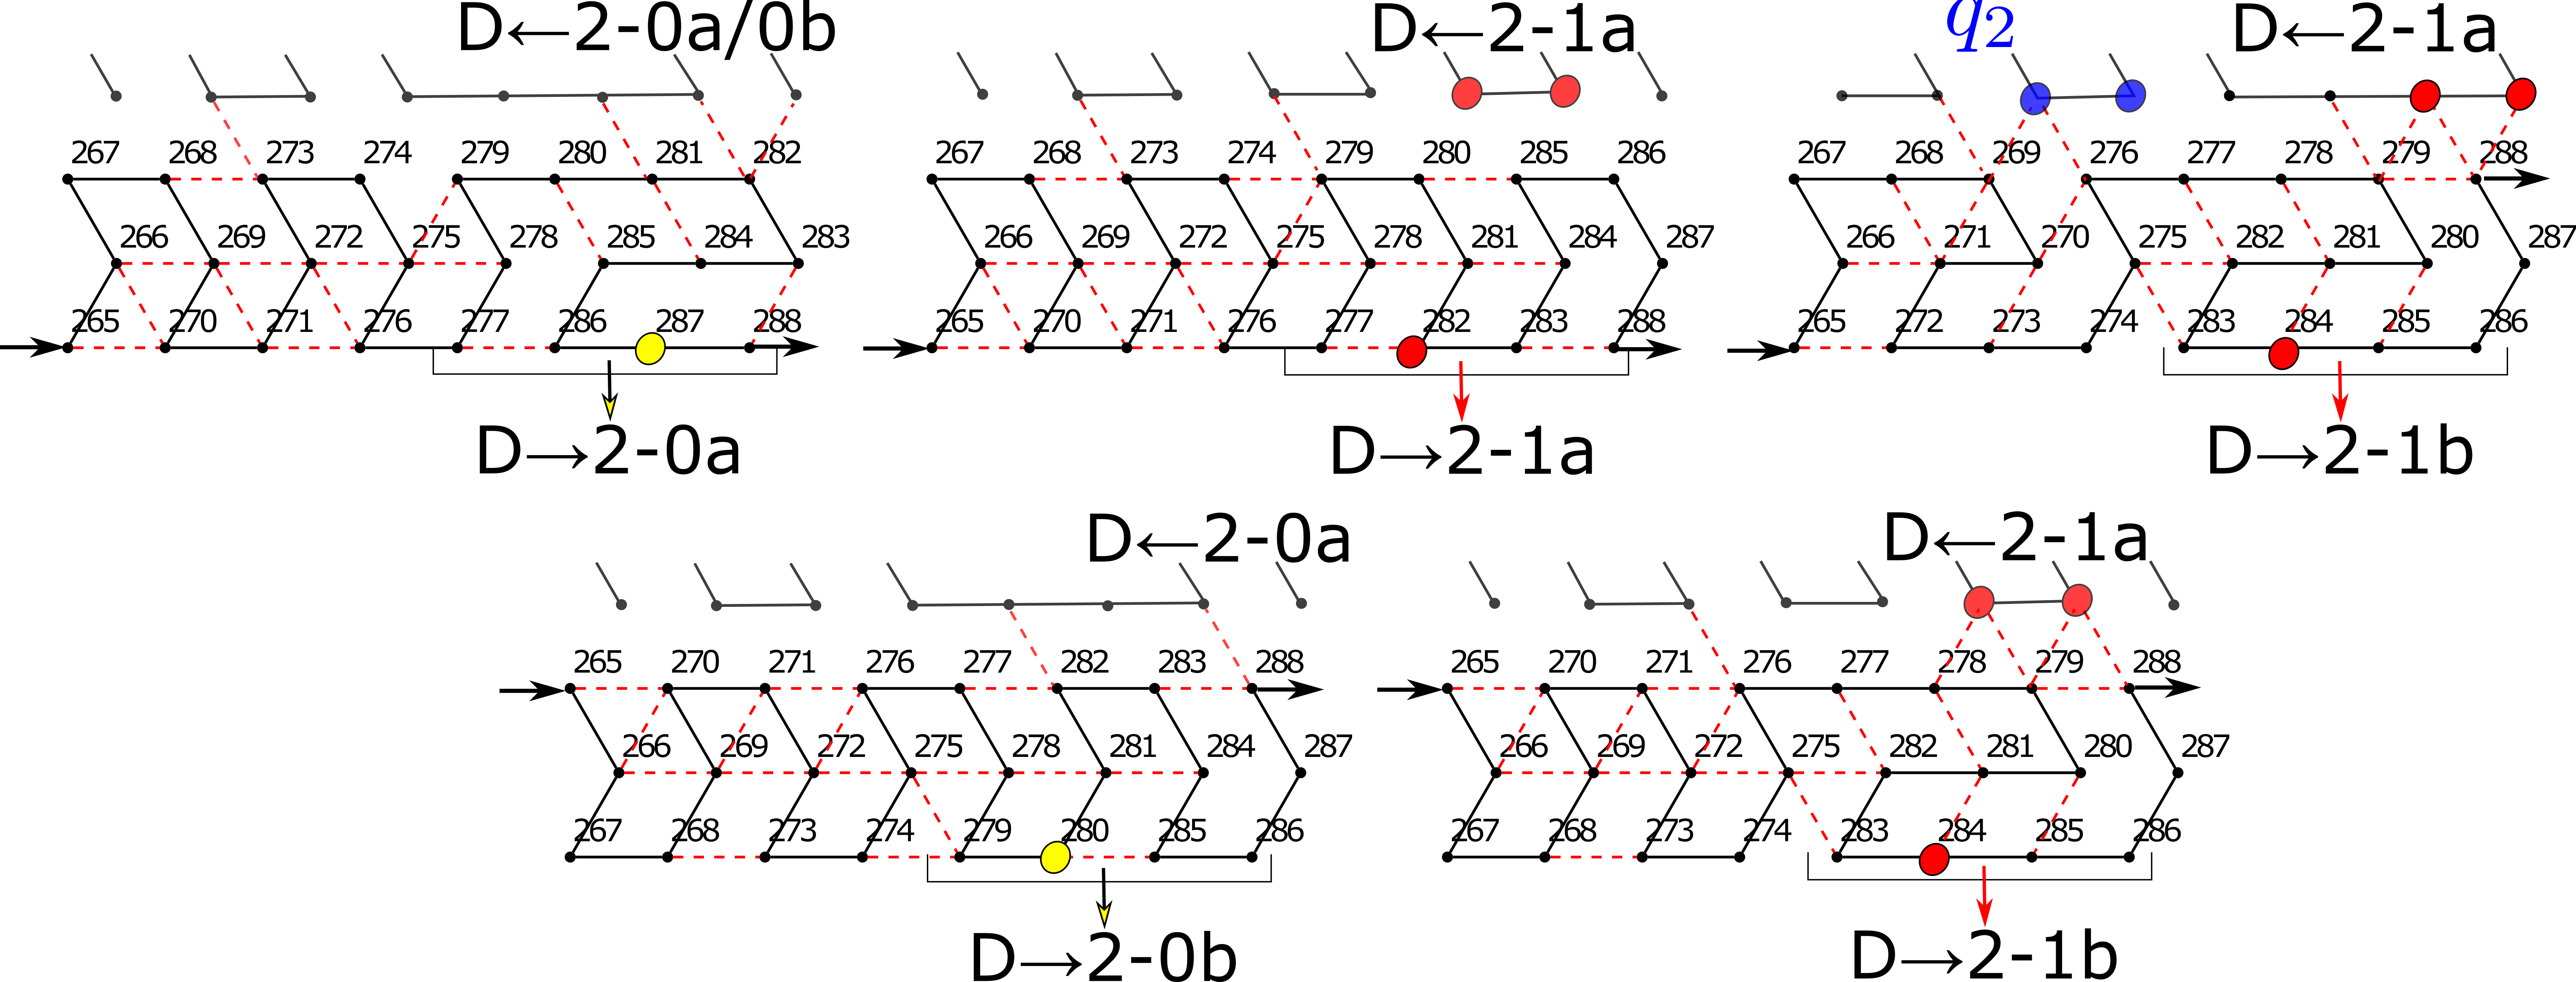
\includegraphics[width=\linewidth]{pic/DFAO-zag2.png}
\caption{The five conformations of DFAO-zag2: (top) Dzag2-L0, Dzag2-L1, Dzag2-T1, (bottom) Dzag2-R0, and Dzag2-R1.
The first and second halves are diverted to implement the body-rgy and body-gx components of the turning module, respectively. 
}
\label{fig:DFAO-zag2}
  \end{figure} 
%%%%%%%%%%%%%%%%%%%%%%%%%%%

In the second zig, $n$ DFAO-zig2s check whether the first 0 is followed (being read from LSB) by 0 or 1, in a similar manner to the search for the first 0.
They usually take one of the two conformations Dzig2-1 and Dzig2-0 to copy 1's and 0's, which start and end at the bottom (see Fig.~\ref{fig:DFAO-zig2}). 
At the encounter to the first 0, a DFAO-zig2 folds into a special conformation Dzig2-f0 and ends at the top. 
The next DFAO-zig2, if any, starts folding at the top so that it takes the special conformation Dzig2-0f0 if the first 0 is followed by 0 or Dzig2-1f0 if it is followed by 1. 
Recall that reading 1 here is equivalent to transitioning to $q_2$ in the DFAO, that is, $P[i] = {\rm L}$. 
Dzig2-1f0 exposes a marker $q_2$ downward. 
These conformations end at the bottom so that the remaining bits are copied by the ordinary conformations Dzig2-1 and -0. 
%They first copy the 1's by the conformation Dzig2-1 (top left in Fig.~\ref{fig:DFAO-zig2}) until the first 0, read from the LSB, which is distinguished from the other 0's by the mark. 
%Starting at the bottom and reading 0, the DFAO-zig2 can take two conformations Dzig2-0 and -f0.
%They share the first half.
%The marker f0 folds the second half so as to end at the top, yielding Dzig2-f0. 
%The next DFAO-zig2 therefore starts to fold at the top so that it takes one of the two conformations Dzig2-f00 and -f01 depending on the bit read.
%Recall that reading 1 here is equivalent to transitioning to $q_2$, that is, $P[i] = L$.
%Observe that Dzig2-f01 is provided with the marker $q_2$, which lets the DFAO-zag2 component below know $P[i] = L$. 
%These conformations end at the bottom.
%The remaining 0's and 1's are copied by Dzig2-0 and -1.
The second zag starts at the bottom and copy 0's and 1's by the two conformations Dzag2-L0 and -L1 of DFAO-zag2 (top left and center in Fig.~\ref{fig:DFAO-zag2}) until a DFAO-zag2 encounters the 1 marked by $q_2$, if any. 
At the encounter, the DFAO-zag2 takes the special conformation Dzag2-T1 and changes the ending position to the top, letting the remaining DFAO-zag2s rather take Dzag2-R0 and -R1 for copying, which end at the top.
As such, the second zag can feed $P[i]$ to PFS as the position of its first bead.

%The third zig lets $P[i]$ go through its AO (or $\overline{\rm AO}$) component to be reinterpreted either as A(cute) or as O(btuse) and propagates the current count $i$.   


%%%%%%%%%%%%%%%%%%%%%%%%%%%%%%%
%-------------------------------------------------------------------------------------------
			\subsubsection{Turning module}
%-------------------------------------------------------------------------------------------

\begin{figure}[t]
\centering
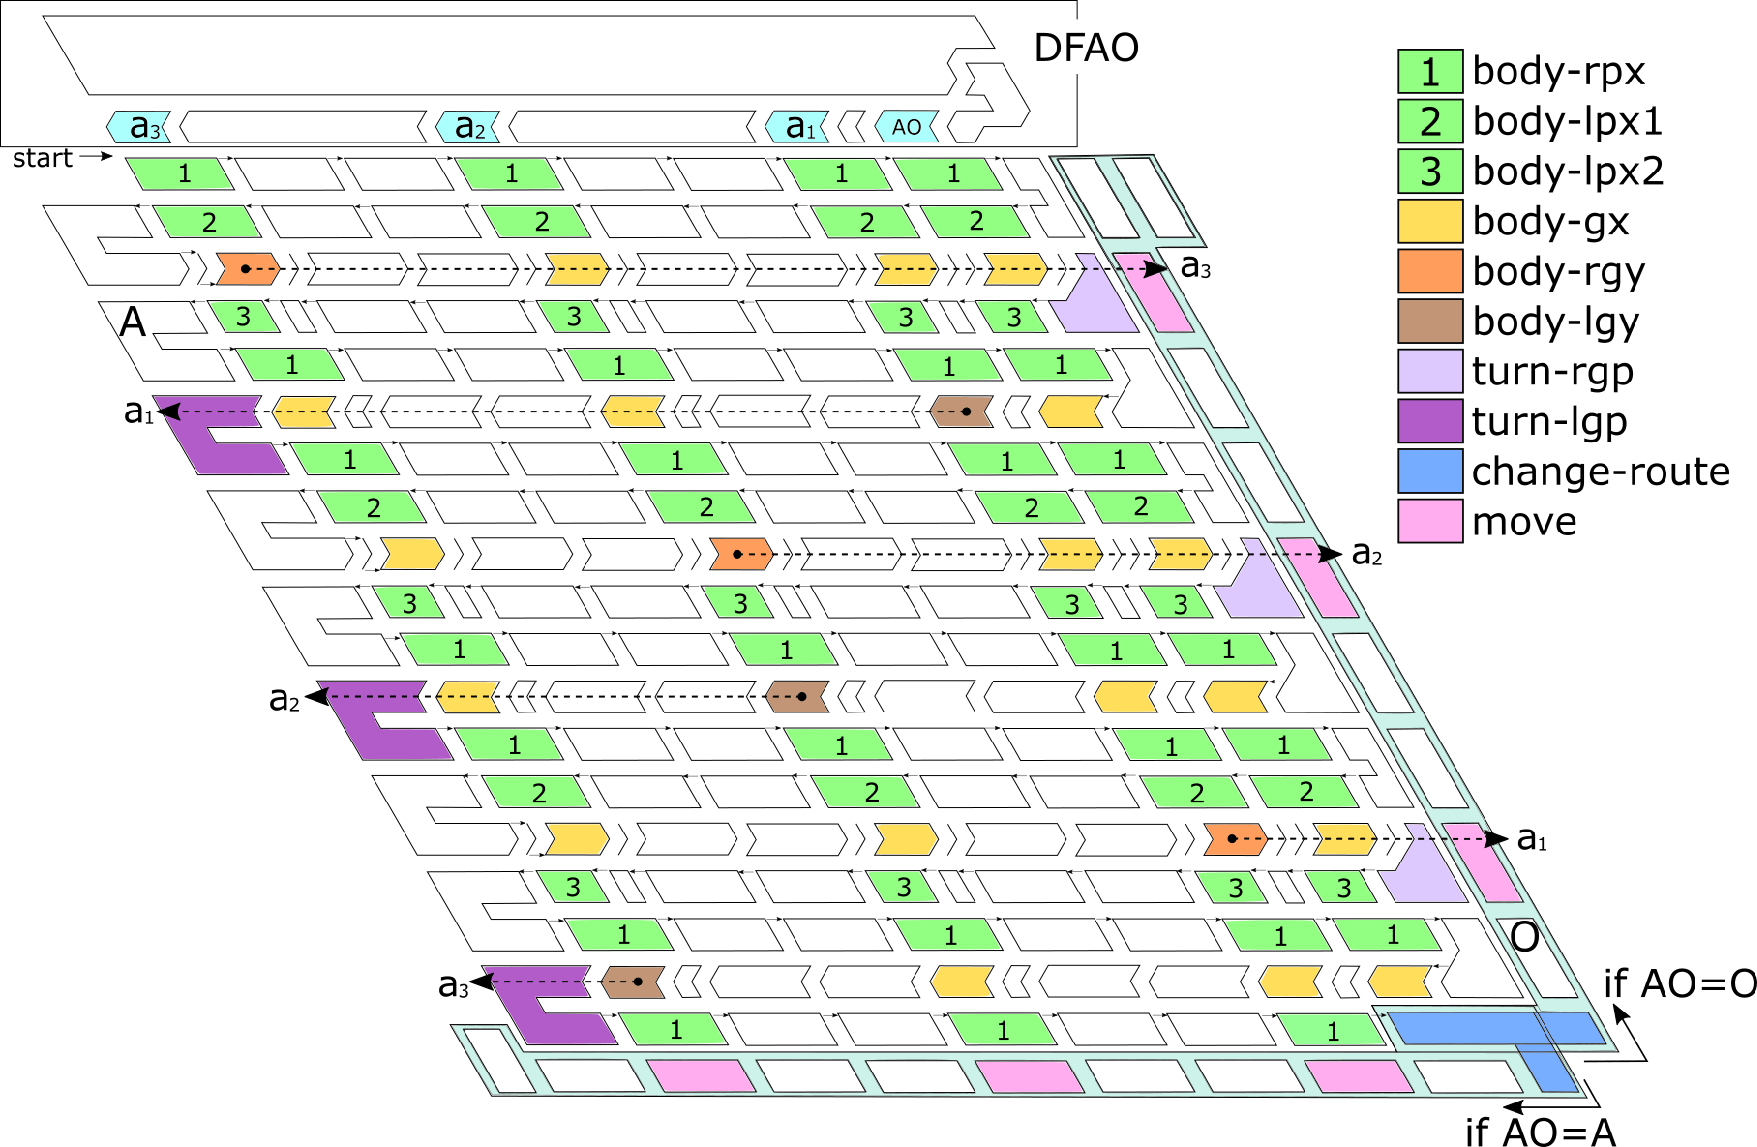
\includegraphics[width=\linewidth]{pic/overall_turn_part.pdf}
\caption{
Component-level abstraction of folding of turning module.
All the white components in the middle are spacers, some of which are implemented in the shape of parallelogram instead of glider. 
 }
\label{fig:overall_turning}
\end{figure}

The last module is for turn. 
It consists of two submodules: bit-sequence bifurcator and steering arm (shaded in light blue in Fig.~\ref{fig:overall_turning}). 

The bifurcator bifurcates the bits of the current count $i$ and the reinterpreted signal (A or O) as shown in Fig.~\ref{fig:abst_dragon} while folding into zigzags.
For that, it employs components to handle the following four types of tasks: 
\begin{enumerate}[itemsep=0pt]
\item propagate 1-bit vertically: body-rpx (Fig.~\ref{fig:body-rpx} (left)), body-lpx1 (Fig.~\ref{fig:body-rpx} (right)), and body-lpx2 (Fig.~\ref{fig:half-adder});
\item let 1-bit cross another 1-bit: body-gx (Fig.~\ref{fig:DFAO-zag2}); 
\item fork 1-bit vertically and horizontally: body-rgy (Fig.~\ref{fig:DFAO-zag2}) and body-lgy (Fig.~\ref{fig:body-lgy});  
\item undergo transition between a zig and a zag and exposes 1-bit outside: turn-rgp (Fig.~\ref{fig:turn-rgp}) and turn-lgp (Fig.~\ref{fig:turn-lgp}). 
\end{enumerate} 
%that propagates 1bit vertically (body-rpx, body-lpx1, and body-lpx2 in Figure~\ref{fig:overall_turning}), that lets 1bit cross another 1bit (body-gx), that forks 1bit vertically and horizontally (body-rgy, body-lgy), and that undergoes transition from a zig to a zag or from a zag to a zig and exposes 1bit outside (turn-rgp, turn-lgp).
Components to handle the first two types of tasks have already been implemented (see, e.g., \cite{HaKiOtSe2016}) so that we shall explain the others.

%The component body-rgy takes one of the two conformations in Figure~\ref{fig:body-rgy} depending on the 1-bit encoded in the two beads above.
%Output below, the 1-bit is encoded as a type of the second bead from left, while output right, it is encoded as the position of its last bead (top or bottom).
%Its zag-variant, body-lgy, is implemented analogously; for its conformations.

%\begin{figure}[h]
\begin{wrapfigure}{r}{0.55\linewidth}
\vspace*{-5mm}
\centering
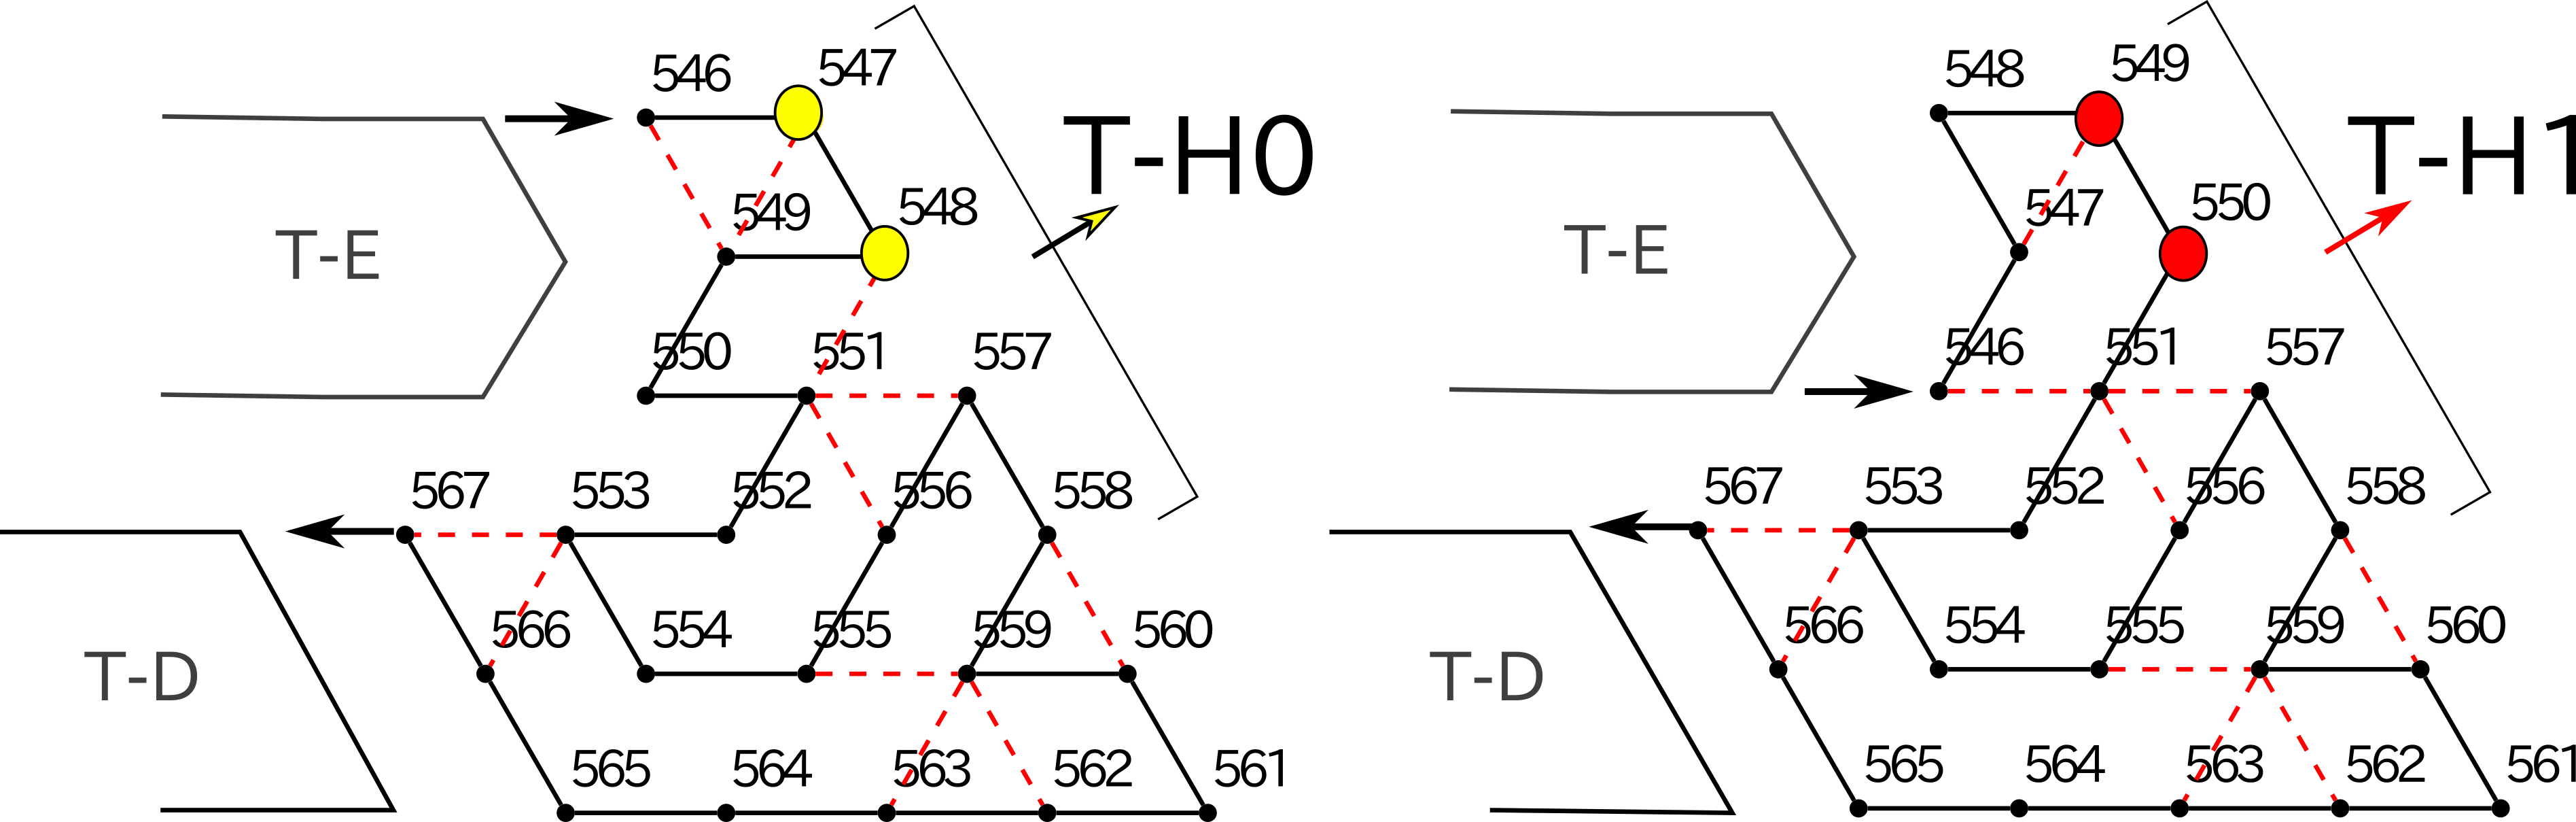
\includegraphics[width=\linewidth]{pic/turn-rgp.png}
\caption{The two conformations of turn-rgp.}
\label{fig:turn-rgp}
\vspace*{-3mm}
\end{wrapfigure}
%\end{figure}

The component body-rgy is implemented by reusing the first half of DFAO-zag2 (Fig.~\ref{fig:DFAO-zag2}). 
Starting from the bottom, it can take two conformations which end at different heights and expose sequences of bead types sufficiently pairwise distinct downward. 
Hence, we can divert it to fork 1bit input rightward and downward. 
The 1bit thus forked transfers till the end of a zag and is converted by the turn-rgp into a sequence of bead types (see Fig.~\ref{fig:turn-rgp}). 
The body-lgy and turn-lgp are their zig counterparts (Figs.~\ref{fig:body-lgy} and \ref{fig:turn-lgp}). 

%The 1bit forked rightward by a body-rgy transfers till the end of the zig without being jammed because all remaining modules in the zig are designed in such a way that they start and end at the same height like the even-distance glider.
%The module turn-rgp receives the 1bit (top or bottom), and exposes it by taking one of the two comformations in Figure~\ref{fig:turn-rgp}.
%The module turn-lgp functions analogously in zags as being folded in Figure~\ref{fig:turn-lgp}.

\begin{figure}[h]
\centering
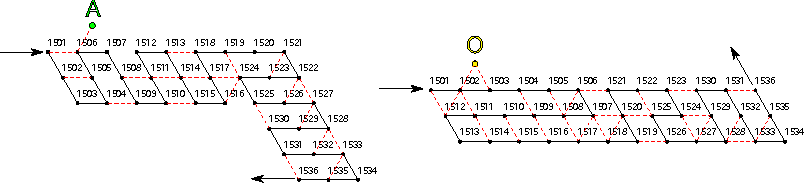
\includegraphics[width=\linewidth]{pic/change_route.pdf}
\caption{The two conformations of change-route.}
\label{fig:change_route}
\end{figure}

The bifurcator also propagates the 1-bit A/O, output by the DFAO module, to tell the steering arm which way it should take.
Specifically, the signal has the component, change-route, of the steering arm take one of the two conformations in Fig.~\ref{fig:change_route}, guiding the rest of the arm towards the specified direction.
The remaining arm is a catenation of move components (Fig.~\ref{fig:move}), which is capable of letting the bifurcated bit sequence through.  
Note that the turning module need not bifurcate AO.
Indeed, the second and third turning modules are supposed to turn in the same manner as the first one.
It hence suffices to append A and O to the bifurcated bit sequences on the acute side and obtuse side, respectively, as shown in Fig.~\ref{fig:overall_turning}.

\begin{remark}
As suggested in Fig.~\ref{fig:overall_turning}, the bifurcation component actually outputs an input bit sequence also downward.
That is, it trifurcates the input.
This provides a more space-efficient way to replicate a bit sequence many-folds.
\end{remark}


%%%%%%%%%%%%%%%%%%%%%%%%%%%%%%%